\documentclass[xcolor=table]{beamer}
\usepackage[UTF8,noindent]{ctexcap}
%\setCJKsansfont[ItalicFont={华文新魏}]{黑体}
\renewcommand\CJKfamilydefault{\CJKsfdefault}
\usepackage{tikz}
\usetikzlibrary{positioning}
\usetheme{PaloAlto}
\usecolortheme{crane}
%\usebeamerfonttheme{professionalfonts}
\usepackage{arev}
\newtheorem{thm}{定理}
\renewcommand\proofname{证明}
%\logo{\includegraphics{HNU_Logo1.png}}

\title{杂谈勾股定理}
\subtitle{数学史讲座之一}
\institute{九章学堂}
\author{Chris}
\date{\today}
\subject{勾股定理}
\keywords{勾股定理,历史}

\begin{document}

\begin{frame}
\titlepage
\end{frame}

\begin{frame}{目录}
\tableofcontents
\end{frame}

\section{勾股定理在古代}
\begin{frame}{古中国数学}{定理发现}
中国在 3000 多年前就知道勾股数的概念,比古希腊更早一些。

《周髀算经》的记载:
\begin{itemize}
\item 公元前 11 世纪,商高答周公问:
\begin{quote}
勾广三,股修四,径隅五。
\end{quote}
\item 又载公元前 7--6 世纪陈子答荣方问,表述了勾股定理的一般形式:
\begin{quote}
若求邪至日者,以日下为勾,日高为股,勾股各自乘,并而开方除之。得邪至日。
\end{quote}
\end{itemize}
\end{frame}

\section{勾股定理在现代}
\begin{frame}{现代叙述}
\begin{thm}[勾股定理]
直角三角形斜边的平方等于两直角边的平方和。

可以用符号语言表述为:设直角三角形 $ABC$,其中$\angle C = 90^{\circ}$,则有
\begin{equation}
AB^{2}=BC^{2}+AC^{2}.
\end{equation}
\begin{center}
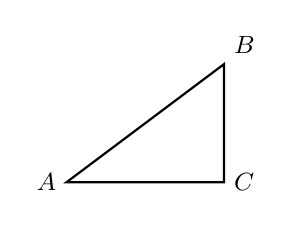
\begin{tikzpicture}[scale=0.5,font=\small]
\draw [thick] (0,0) node [left] {$A$}
    -- (4,0) node [right] {$C$}
    -- (4,3) node [above right] {$B$}  -- cycle;
%\draw (3.5,0)  |-- (4,0.5); %该句语法错误?
\end{tikzpicture}
\end{center}
\end{thm}
\end{frame}

\begin{frame}
% 颜色 craneorange 是在 crane 色彩主题中定义的
\rowcolors{2}{craneorange!25}{craneorange!50}
\begin{tabular}{rrr}
\rowcolor{craneorange}直角边 $a$ & 直角边$b$ & 斜边 $c$\\
3 & 4 & 5 \\
5 & 12 & 13\\
7 & 24 & 25\\
8 & 15 & 17\\
\end{tabular}
\end{frame}

\end{document}
